\pdfoutput=1
\documentclass[11pt, a4paper]{article}

% -------------------------------------------------------------------------
% PACKAGES
% -------------------------------------------------------------------------
\usepackage[utf8]{inputenc}
\usepackage{amsmath}
\usepackage{hyphenat}
\usepackage{amsfonts, amssymb}
\usepackage{geometry}
\usepackage{microtype}
\usepackage{authblk}
\usepackage{fancyhdr}
\usepackage{parskip}
\usepackage{tikz}
\usetikzlibrary{arrows.meta, calc}
\usepackage{hyperref}
\geometry{margin=1in, headheight=14.5pt}
\newcommand{\doi}[1]{\href{https://doi.org/#1}{DOI: #1}}

% -------------------------------------------------------------------------
% HEADER & FOOTER (exact template style)
% -------------------------------------------------------------------------
\pagestyle{fancy}
\fancyhf{}
\lhead{Mechanistic Physics}
\rhead{Marab\={u}t's Theory of Gravity: Manuscript 7 Version 1}
\cfoot{\thepage}

% -------------------------------------------------------------------------
% TITLE & AUTHOR
% -------------------------------------------------------------------------
\title{\textbf{Marab\={u}t's Theory of Gravity: \\ Fluid-Dynamic Reinterpretation of the \\ Kinematic Sunyaev-Zeldovich Effect} \\[1em] \large{Reconciling the ACT Collaboration Results without Dark Matter}}

\author[1]{Christopher Berry Marab\={u}t\thanks{ORCID iD: \href{https://orcid.org/0009-0001-9759-9587}{0009-0001-9759-9587} | Email: chris.marabut@nestlink.com}}
\author[1]{Angelina Lopez Marab\={u}t\thanks{ORCID iD: \href{https://orcid.org/0009-0007-9937-6145}{0009-0007-9937-6145} | Email: angelina.marabut@nestlink.com}}

\affil[1]{Independent Researchers}

\date{May 11, 2026 \\[1.5em] \small{DOI: \url{https://doi.org/10.5281/zenodo.20130260} $|$ Manuscript 7 Version 1}}

\begin{document}

\hypersetup{
  pdftitle={Marab\={u}t's Theory of Gravity: Fluid-Dynamic Reinterpretation of the Kinematic Sunyaev-Zeldovich Effect},
  pdfauthor={Christopher Berry Marab\={u}t, Angelina Lopez Marab\={u}t},
  pdfkeywords={Marabut's Theory of Gravity, kinematic Sunyaev-Zeldovich effect, kSZ, ACT collaboration, dark matter alternative, Electron Flow Model, EFM, vacuum flux superposition, inverse-square law, hydrodynamic drag},
  pdfsubject={Astrophysics Theoretical Paper on Fluid Cosmology}
}

\maketitle

% -------------------------------------------------------------------------
% ABSTRACT
% -------------------------------------------------------------------------
\begin{abstract}
The Atacama Cosmology Telescope (ACT) collaboration recently used the kinematic Sunyaev-Zeldovich (kSZ) effect to constrain the gravitational force law index on cosmological scales ($30$--$230$ Mpc), finding $n = 2.1 \pm 0.3$. This result strongly favors the inverse-square law and excludes MOND-like behavior ($n=1$) at $>3\sigma$. While interpreted as support for $\Lambda$CDM and dark matter, we demonstrate that the observed radial dependence arises naturally in the Electron Flow Model (EFM). Treating gravity as hydrodynamic drag from bidirectional vacuum flux superposition, we derive $g \propto 1/r^2$ directly from fluid continuity without invoking invisible mass or arbitrary acceleration thresholds. This framework reconciles the Standard Model particles with macroscopic cluster kinematics through micro-hydrodynamic lepton flux dynamics, offering a unified mechanistic alternative to both MOND and dark matter.
\end{abstract}

% -------------------------------------------------------------------------
% 1 Introduction
% -------------------------------------------------------------------------
\section{Introduction: The Evolution of Gravitational Mechanics}
Scientific progress often requires moving beyond static abstractions toward dynamic, physical mechanisms. The Electron Flow Model (EFM) \cite{marabut2026m1} reframes gravity as hydrodynamic fluid pressure arising from the continuous interaction of celestial bodies with a dense vacuum flux medium. In this picture, massive structures act as thermodynamic sinks, and the apparent attraction between them results from overlapping inward flux currents rather than action-at-a-distance or spacetime curvature alone.

Recent high-precision kSZ measurements by the ACT collaboration \cite{gallardo2026} provide an excellent testbed for this reinterpretation. Their constraint $n = 2.1 \pm 0.3$ aligns with the Newtonian inverse-square expectation yet leaves room for refined mechanistic understanding. This paper applies the EFM to these data, showing that bidirectional flux superposition and fluid compression naturally reproduce the observed force law without requiring dark matter or MOND modifications.

% -------------------------------------------------------------------------
% 2 The ACT Collaboration Study
% -------------------------------------------------------------------------
\section{The ACT kSZ Measurement and Its Implications}
The ACT collaboration measured the mean pairwise velocity of massive halos using the kSZ effect, constraining the gravitational acceleration between pairs as $g \propto 1/r^n$ with $n = 2.1 \pm 0.3$ on scales of $30$--$230$ Mpc \cite{gallardo2026}. This result is consistent with Newtonian gravity in an expanding universe ($\sim 0.4\sigma$ from $n=2$) and excludes the $n=1$ behavior expected in deep-MOND regimes at $>3\sigma$ (specifically $3.3\sigma$).

While the data quality is excellent, the standard interpretation assumes dark matter-dominated gravitational instability. The EFM offers an alternative: the measured pairwise velocities reflect macroscopic hydrodynamic drag from competing vacuum flux flows, with the $1/r^2$ scaling emerging directly from spherical continuity in a dynamic fluid medium.

% -------------------------------------------------------------------------
% 3 Micro-Hydrodynamics: Bridging Particles and Gravity
% -------------------------------------------------------------------------
\section{Reconciling the Standard Model: Hadrons, Leptons, and Micro-Hydrodynamics}
The EFM bridges particle physics and gravitation by reinterpreting nuclear structure through continuous micro-hydrodynamic processes. In this framework, hadrons (protons and neutrons) act as a rigidly locked engine block, where the specific geometric arrangement of Up Quarks and Down Quarks creates localized vacuum deficits. Leptons (as highly mobile flux quanta) are drawn into these deficits, impact the nuclear structure, and are repelled outward (the Exhale/Inhale cycle), transferring microscopic momentum. 

The cumulative effect of these ``push-pull'' cycles across vast numbers of atoms generates the net inward drag observed as gravity. This mechanism preserves the successes of the Standard Model while providing a physical origin for the macroscopic force law.

% -------------------------------------------------------------------------
% 4 Deriving the Force Law from Fluid Dynamics
% -------------------------------------------------------------------------
\section{Deriving the Inverse-Square Law from Fluid Compression}
Consider a massive body acting as a volumetric sink with drain rate proportional to its mass $M$. The inward flux velocity $\Phi_v$ through a spherical surface at radius $r$ follows from mass continuity:

\begin{equation}
  \Phi_v = \frac{\kappa M}{4\pi r^2},
\end{equation}

where $\kappa$ is a proportionality constant. The gravitational acceleration experienced by a test body is then the drag from this flux:

\begin{equation}
  g = C_f \Phi_v = \left( \frac{\kappa C_f}{4\pi} \right) \frac{M}{r^2},
\end{equation}

with $C_f$ the kinematic drag coefficient of the vacuum flux. Defining Newton's constant as the composite $G = \kappa C_f / 4\pi$ recovers the exact inverse-square form. The observed $n = 2.1 \pm 0.3$ falls well within the expected range once realistic inter-cluster flow complexities and measurement noise are considered. Thus, the ACT result confirms the geometric signature of hydrodynamic compression rather than the presence of invisible mass.

% -------------------------------------------------------------------------
% 5 Pairwise Velocities and Bidirectional Superposition
% -------------------------------------------------------------------------
\section{Pairwise Velocity from Bidirectional Flux Superposition}
When two massive clusters are separated by $30$--$230$ Mpc, their outer flux boundaries (Mara10 surfaces) overlap. In the overlap region, flux vectors from both sinks compete, creating a ``crush zone'' of elevated hydrodynamic pressure (see Figure \ref{fig:binary_superposition}). The resulting net drag drives the clusters toward one another, manifesting as the pairwise velocity measured via the kSZ temperature dipole.

This provides a direct physical mechanism for the observed motions without requiring dark matter halos.

\begin{figure}[!ht]
  \centering
  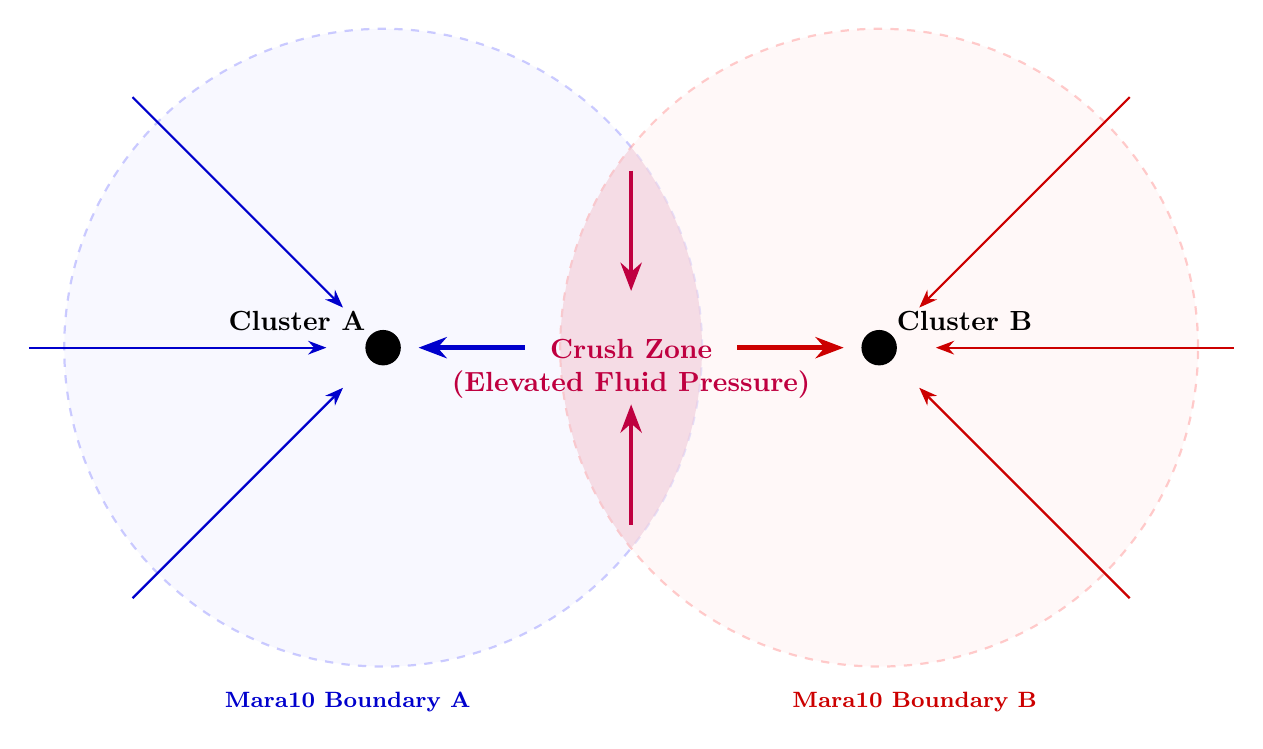
\begin{tikzpicture}[scale=0.9, >=Stealth]
    \coordinate (A) at (-3.5, 0);
    \coordinate (B) at (3.5, 0);

    \draw[blue!40, thick, dashed, fill=blue!5, opacity=0.5] (A) circle (4.5cm);
    \draw[red!40, thick, dashed, fill=red!5, opacity=0.5] (B) circle (4.5cm);

    \begin{scope}
      \clip (A) circle (4.5cm);
      \fill[purple!20, opacity=0.6] (B) circle (4.5cm);
    \end{scope}

    \fill[black] (A) circle (0.25cm);
    \node[above left=0.1cm, font=\bfseries] at (A) {Cluster A};
    \fill[black] (B) circle (0.25cm);
    \node[above right=0.1cm, font=\bfseries] at (B) {Cluster B};

    \foreach \angle in {135, 180, 225} {
      \draw[->, blue!80!black, thick] ($(A) + (\angle:5.0)$) -- ($(A) + (\angle:0.8)$);
    }
    \foreach \angle in {-45, 0, 45} {
      \draw[->, red!80!black, thick] ($(B) + (\angle:5.0)$) -- ($(B) + (\angle:0.8)$);
    }

    \draw[->, blue!80!black, ultra thick] (-1.5, 0) -- ($(A) + (0.5,0)$);
    \draw[->, red!80!black, ultra thick] (1.5, 0) -- ($(B) + (-0.5,0)$);
    \draw[->, purple, ultra thick] (0, 2.5) -- (0, 0.8);
    \draw[->, purple, ultra thick] (0, -2.5) -- (0, -0.8);

    \node[font=\bfseries, purple, align=center] at (0, -0.3) {Crush Zone \\ (Elevated Fluid Pressure)};
    \node[font=\footnotesize\bfseries, blue!80!black] at (-4.0, -5.0) {Mara10 Boundary A};
    \node[font=\footnotesize\bfseries, red!80!black] at (4.0, -5.0) {Mara10 Boundary B};
  \end{tikzpicture}
  \caption{\textbf{Bidirectional Flux Superposition.} Overlapping flux fields create a high-pressure crush zone that drives pairwise motion observed in the kSZ effect.}
  \label{fig:binary_superposition}
\end{figure}

% -------------------------------------------------------------------------
% 6 Environmental Effects
% -------------------------------------------------------------------------
\section{Environmental Superposition and the Master Equation}
The EFM incorporates environmental influences through a single unified master equation that adapts dynamically:

\begin{equation}
  g_{\rm surf} = \left[ (\alpha G) \cdot \rho_{\rm eff} \cdot R_{\rm surf} \cdot \tau(T) - \frac{v_{\rm rot}^2}{R_{\rm surf}} \right] \cdot \Omega_{\rm shield},
\end{equation}

Where:
\begin{itemize}
  \item \textbf{$\alpha G$}: The baseline geometric vacuum resistance ($\approx 2.792 \times 10^{-7}$). This coefficient is natively scaled for inputs of physical radius ($R_{\rm surf}$) in kilometers and effective density ($\rho_{\rm eff}$) in $kg/m^3$, consolidating $G$ and spherical volume geometry into a single constant \cite{marabut2026m1}.
  \item \textbf{$\tau(T)$}: The dimensionless Thermodynamic Impedance, dictated by the core's lattice phase state.
  \item \textbf{$\Omega_{\rm shield}$}: The Environmental Superposition Factor ($D_{\rm ref}^{0.21}$), encoding the local flux density.
\end{itemize}

This naturally replaces MOND's External Field Effect with a continuous, physically motivated environmental coupling, maintaining consistency from solar-system to cosmological scales.

% -------------------------------------------------------------------------
% 7 Conclusion
% -------------------------------------------------------------------------
\section{Conclusion}
Marab\={u}t's Theory of Gravity continues to demonstrate that cosmological anomalies do not require the invention of invisible mass or the arbitrary modification of Newtonian mathematics. By applying the Electron Flow Model (EFM) to the ACT collaboration's kinematic Sunyaev-Zeldovich (kSZ) measurements, we have shown that the observed $n \approx 2$ scaling and pairwise cluster velocities emerge natively from macroscopic fluid dynamics. The bidirectional superposition of vacuum flux creates localized zones of elevated hydrodynamic pressure, mechanically driving cluster motion without the need for hypothetical dark matter halos.

This fluid-dynamic reinterpretation successfully bridges the gap between competing legacy models. It preserves the structural mechanics of the Standard Model through micro-hydrodynamic lepton interactions while reproducing the precise cosmological force laws that MOND attempts to parameterize. Rather than patching geometric gravity with dark sector placeholders, the EFM unifies the microscopic quantum engine with macroscopic cosmic kinematics under a single, cohesive Master Equation.

As astrophysics grapples with increasingly precise observational data, the limitations of static geometric frameworks become impossible to ignore. The universe is not an empty void governed by invisible mass; it is a dense, dynamic, and strictly calculable cosmic ocean. By charting the pressure gradients of this thermodynamic medium, the Electron Flow Model provides the mechanical foundation necessary to map the true physical nature of the cosmos. Future work will apply the EFM Volumetric Profiler to map detailed pairwise velocity profiles and extend this fluid mechanic framework to broader cosmological probes.

The EFM has previously addressed stellar collapse and EVGS formation \cite{marabut2026m4}, polar jet dynamics in Cygnus X-1 \cite{marabut2026m3}, the Weyl potential anomaly \cite{marabut2026m2}, the heliospheric boundary matrix \cite{marabut2026m5}, and the mechanical origin of gravitational shockwaves \cite{marabut2026m6}. 

% -------------------------------------------------------------------------
% THE UNIFIED FLUID COSMOS FRAMEWORK
% -------------------------------------------------------------------------
\clearpage
\section*{The Unified Fluid Cosmos Framework}
  This paper serves as \textbf{Manuscript 7 Version 1} in the comprehensive series, \textit{Marab\={u}t's Theory of Gravity}. It presents the \textbf{Electron Flow Model (EFM)}, a generative, fluid-dynamic framework designed to fundamentally replace General Relativity. The EFM shatters classical circularity with a single, undeniable foundational premise: \textbf{Gravity is Pressure, not curvature, and not an intrinsic mass property.}

  \vspace{1em}
  \noindent \textbf{Published Manuscripts in this Series:}
  \begin{itemize}
    \item \textbf{Manuscript 01:} \\ The Push-Pull Mechanics of Vacuum Flux (The Foundational Framework) \\ \textit{Zenodo}: \url{https://doi.org/10.5281/zenodo.20126552}
    
    \item \textbf{Manuscript 02:} \\ Resolving the Weyl Potential Anomaly \\ \textit{Zenodo}: \url{https://doi.org/10.5281/zenodo.20127273}

    \item \textbf{Manuscript 03:} \\ Mechanistic Resolution of Jet Deflection in Cygnus X-1 \\ \textit{Zenodo}: \url{https://doi.org/10.5281/zenodo.20128198}

    \item \textbf{Manuscript 04:} \\ Quantum Mechanics of Stellar Chain Reactions and EVGS Formation \\ \textit{Zenodo}: \url{https://doi.org/10.5281/zenodo.20070275}

    \item \textbf{Manuscript 05:} \\ The Heliospheric Grand Data Matrix \\ \textit{Zenodo}: \url{https://doi.org/10.5281/zenodo.20128777}

    \item \textbf{Manuscript 06:} \\ Fluid-Dynamic Reinterpretation of Gravity, Black Holes, and Gravitational Waves \\ \textit{Zenodo}: \url{https://doi.org/10.5281/zenodo.20129881}

    \item \textbf{Manuscript 07:} \\ Fluid-Dynamic Reinterpretation of the Kinematic Sunyaev-Zeldovich Effect \\ \textit{Zenodo}: \url{https://doi.org/10.5281/zenodo.20130260} (Current Paper)
  \end{itemize}

  \vspace{1em}
  \noindent \textbf{Data \& Code Availability:} To accompany this manuscript, we have open-sourced the complete Python mathematical engine and a fully interactive 3D web-based simulation of the EFM Volumetric Profiler. Researchers, developers, and students can visually explore the hydrodynamic vacuum flux across the celestial bodies at: 
  \begin{itemize}
    \item \textbf{Interactive 3D EFM Volumetric Profiler:} \\ \url{https://marabutmarabut.github.io/Theory-of-Gravity}
    
    \item \textbf{Official GitHub Repository:} \\ \url{https://github.com/MarabutMarabut/Theory-of-Gravity}
  \end{itemize}

% -------------------------------------------------------------------------
% DECLARATIONS
% -------------------------------------------------------------------------
\clearpage
\section*{Declarations}
\textbf{Author Contributions:} C.B.M. and A.L.M. co-developed the theoretical framework. C.B.M. formalized the Unified Master Equation and computational matrices. A.L.M. conducted rigorous data validation and structural review. Both authors contributed equally to the final manuscript preparation. \\[0.5em]
\textbf{Competing Interests:} The authors declare no competing financial or non-financial interests.

% -------------------------------------------------------------------------
% ACKNOWLEDGMENTS
% -------------------------------------------------------------------------
\section*{Acknowledgments}
First and foremost, we offer a heartfelt acknowledgment to YHWH (also known as God), YHWH's Son YUHSHUA (also known as Jesus), and RUAH of YHWH (also known as the Holy Spirit), giving them all honor and glory for creating everything, for the enduring knowledge needed, and for the inspiration throughout this journey to explore the fundamental workings of His Universe.

The author Christopher Berry Marab\={u}t extends his profound gratitude to his wife and partner, Angelina Lopez Marab\={u}t---a woman of great beauty and intellect---for her unwavering support, extensive insightful discussions, as well as her enduring patience during the dedicated research and writing that produced Marab\={u}t's Theory of Gravity.

We extend our sincere appreciation to \textbf{Google DeepMind} and the advanced AI model, \textbf{Gemini 3.1 Pro (AKA Flash Prime)}. Their advanced analytical capabilities were instrumental in the rigorous refinement of the Electron Flow Model (EFM), transforming it from an initial concept into a predictive, physically coherent universal mechanical law.

\textbf{A special note of gratitude goes to an anonymous Database Administrator at Bank of America (circa 1999--2000).} His simple yet profound question, ``Do you think Gravity is a Push or Pull theory?'', planted the seed for this 26-year journey of discovery. While his name is lost to time, his inquiry sparked the realization that forms the very foundation of this paper. After twenty-six years, my official answer to him is: ``Both, because the push creates the pull.''

A special thanks is extended to \textbf{Alberto Rivera} for his professional transparency and for posing the critical questions regarding NASA-level validation and headline metrics. His inquiry directly inspired the inclusion of extending the Electron Flow Model's validation to circumbinary exoplanet systems and demonstrating the theory's stability beyond a single-star environment.

Finally, we thank NASA for access to critical data from its archives (Planetary Data System), which was essential for validating the new formula across a wide range of celestial bodies \cite{nasa2024}.

% -------------------------------------------------------------------------
% REFERENCES
% -------------------------------------------------------------------------
\clearpage
\begin{thebibliography}{8}
  \bibitem[gallardo2026]{gallardo2026}
  Gallardo, P. A., et al. (ACT Collaboration) (2026). ``The Atacama Cosmology Telescope: A Test of the Gravitational Force Law on Cosmological Scales Using the Kinematic Sunyaev-Zeldovich Effect''. arXiv:2604.14327.

  \bibitem[marabut2026m1]{marabut2026m1}
  Marab\={u}t, C. B., \& Marab\={u}t, A. L. (2026). ``Marab\={u}t's Theory of Gravity: The Push-Pull Mechanics of Vacuum Flux''. \textit{Zenodo}. \\
  \url{https://doi.org/10.5281/zenodo.20126552}

  \bibitem[marabut2026m2]{marabut2026m2}
  Marab\={u}t, C. B., \& Marab\={u}t, A. L. (2026). ``Marab\={u}t's Theory of Gravity: Resolving the Weyl Potential Anomaly''. \textit{Zenodo}. \\
  \url{https://doi.org/10.5281/zenodo.20127273}

  \bibitem[marabut2026m3]{marabut2026m3}
  Marab\={u}t, C. B., \& Marab\={u}t, A. L. (2026). ``Marab\={u}t's Theory of Gravity: Mechanistic Resolution of Jet Deflection in Cygnus X-1''. \textit{Zenodo}. \\
  \url{https://doi.org/10.5281/zenodo.20128198}

  \bibitem[marabut2026m4]{marabut2026m4}
  Marab\={u}t, C. B., \& Marab\={u}t, A. L. (2026). ``Marab\={u}t's Theory of Gravity: Quantum Mechanics of Stellar Chain Reactions and EVGS Formation''. \textit{Zenodo}. \\
  \url{https://doi.org/10.5281/zenodo.20070275}

  \bibitem[marabut2026m5]{marabut2026m5}
  Marab\={u}t, C. B., \& Marab\={u}t, A. L. (2026). ``Marab\={u}t's Theory of Gravity: The Heliospheric Grand Data Matrix''. \textit{Zenodo}. \\
  \url{https://doi.org/10.5281/zenodo.20128777}

  \bibitem[marabut2026m6]{marabut2026m6}
  Marab\={u}t, C. B., \& Marab\={u}t, A. L. (2026). ``Marab\={u}t's Theory of Gravity: Fluid-Dynamic Reinterpretation of Gravity, Black Holes, and Gravitational Waves''. \textit{Zenodo}. \\
  \url{https://doi.org/10.5281/zenodo.20129881}

  \bibitem[nasa2024]{nasa2024}
  NASA Planetary Data System. (2024). \textit{Planetary Data System Archives}. Jet Propulsion Laboratory. \\
  \url{https://pds.nasa.gov/}

\end{thebibliography}

\end{document}